\documentclass[a4paper, 12pt]{article}
\usepackage[pdftex, hidelinks]{hyperref}

\usepackage{bm}
\usepackage[T1]{fontenc}
\usepackage[utf8]{inputenc}
\usepackage{algorithmic}
\usepackage{algorithm}
\usepackage{amsfonts}
\usepackage{amssymb}
\usepackage{courier}
\usepackage{booktabs}
\usepackage{graphicx}
\usepackage{listings}
\usepackage{mathtools}
\usepackage{amssymb}
\lstset{basicstyle=\footnotesize\ttfamily,
breakatwhitespace = false,
breaklines = true,
keepspaces = true,
language = R,
showspaces = false,
showstringspaces = false,
belowcaptionskip = \bigskipamount,
framerule = 0.80pt,
frame = tb,
belowskip = \bigskipamount,
escapeinside={<@}{@>}}

\title{TDDE01 -- Machine Learning \\
Laboration Report 5}
\author{{Martin Estgren \texttt{<mares480>}} \\
{Linköping University (LiU), Sweden}}

\begin{document}
\pagenumbering{arabic}
    \maketitle % Generate.

    Increasing the accuracy of \emph{weather forecasts} is an important task. We propose an estimator which produces the \emph{air temperature forecast} in \emph{Sweden}, given a \emph{latitude/longitude coordinate} and also \emph{date}. Some observations by \emph{SMHI}, taken from weather stations, have been given for training our estimator.

    By using a \emph{Nadaraya–Watson regression kernel}, we can estimate the temperatures \(\bm{y'}\). This is done by taking the \emph{kernels} \(k_\sigma(\bm{x}^{(i)}, \bm{x'})\) for each \(i^{th}\) data from the training set and using it as a \emph{weight} when considering the response variable \(\bm{y}^{(i)}\). Essentially, the kernel \(k_\sigma(\bm{x}^{(i)}, \bm{x'})\) will reduce \(\bm{y}^{(i)}\)'s significance in the \emph{total contribution} by giving less weight when the \(\bm{x^{(i)}}\) and \(\bm{x'}\) are further away (in some measure).

    We have used a \emph{Gaussian Radial Basis Function} as our \emph{kernel}, which is defined in Equation~\ref{eq:grbf} below. Note the parameter \(\sigma\), which can be considered as the \emph{spread} or \emph{width} of the kernel, and also \(\bm{x^{(i)}} - \bm{x'}\) which is the \emph{distance function}; giving our kernel the property of a \emph{similarity function} (because of \(e^{(\cdots)}\)).

    By using \(k_\sigma(\bm{x}^{(i)}, \bm{x'})\) in \emph{Nadaraya–Watson's} \(\bm{y'}\) estimator, shown in Equation~\ref{eq:nadaraya_watson}, we are essentially \emph{weighing} how important the contributions from \(\bm{y}^{(i)}\) are to \(\bm{y'}\), because \emph{similar} \(\bm{x}^{(i)}\) will give higher \(k_\sigma\). Further descriptions: see \emph{Friedman et al.\ }~\cite{friedman2009elements}.

    \begin{equation} \label{eq:grbf}
    k_\sigma(\bm{x}, \bm{x'}) = \mathrm{exp}\bigg(\frac{- \, {\left\Vert(\bm{x} - \bm{x'}) \right\Vert}^2}
    {2\sigma^2 \; \{\sigma \approx h\}}\bigg)
    \end{equation}

    \lstinputlisting[firstline=23,lastline=25]{../share/script.r}

    \begin{equation} \label{eq:nadaraya_watson}
    \bm{y'}(\bm{x}, \bm{x'}) = \frac{\sum_n{\bm{y}^{(i)}k_\sigma(\bm{x}^{(i)}, \bm{x'})}}
    {\sum_n{k_\sigma(\bm{x}^{(i)}, \bm{x'})}}
    \end{equation}

    We now describe the functions which were used to determine the distance/similarity for the kernels.

    Below follows the applied \emph{distance functions}, which give the measured distance between a pair of \emph{locations}, \emph{times of the day}, and also \emph{dates of year}. These distance and kernel functions can be found in Listing~\ref{lst:forecast}, where they follow similarly as described.

    \begin{equation*} \label{eq:location}
    d_l = r\, \mathrm{hav}^{-1}(h),\; \mathrm{hav}(\varphi) = \frac{1 - \cos\varphi}{2}
    \end{equation*}
    
    \lstinputlisting[firstline=28,lastline=32]{../share/script.r}
    
    \begin{equation*} \label{eq:time}
    d_t = \begin{cases}
    |x - y| & |x - y| < (x + y) \bmod 24\\
    (x + y) \bmod 24 & |x - y| \geq (x + y) \bmod 24
    \end{cases}
    \end{equation*}

   \lstinputlisting[firstline=45,lastline=51]{../share/script.r}

    \begin{equation*} \label{eq:day}
    d_d = \begin{cases}
    |x - y| & |x - y| < (x + y) \bmod 365\\
    (x + y) \bmod 365 & |x - y| \geq (x + y) \bmod 365
    \end{cases}
    \end{equation*}

   \lstinputlisting[firstline=35,lastline=42]{../share/script.r}
    

    Finally, we have the \emph{three different kernels} which contribute in unison to the final \emph{forecast kernel}. Each of these use Equation~\ref{eq:grbf} with their respective \emph{distance functions} and also \emph{kernel width} \(h\) (\(\sigma\) here).

	An obvious question the reader has by now has: \textit{What values should be assigned to \(2\sigma^2\)?}\newline If said reader does not wonder about this, said reader needs to be more intellectually involved in this papers reasoning in the future. However, the answer to the question has to do with the scale of the range of values that the distance can have. One could assign 1 to as a weight, and it might be sufficient, especially if the values are not very large for relatively close observations. This means it is completely related to the context. When in the the context of physical distance it is reasonable to use 1000000 as \textit{h} since if the point of interest is only a few km away from an already existing observation, the kernel value will return close to 0 values. For date and time, the values already seems to be good enough and only needs to be modified with very small factors. Date uses 3 for \textit{h} and time uses 2. The intuition seems to be confirmed when observing the result from the kernels presented in figure \ref{fig:time}, \ref{fig:dist} and \ref{fig:date}. 

    \section{Result}

    The date and time formats for the data set required pre-processing before they could be used in the above mentioned functions.
    \lstinputlisting[firstline=104,lastline=108]{../share/script.r}


    \begin{figure}[H]
    \centering
    \caption{Distance plot (time of day) for the observations (Ordered by time of day) \label{fig:time}}
	    \begin{minipage}[]{0.2\textwidth}
	    	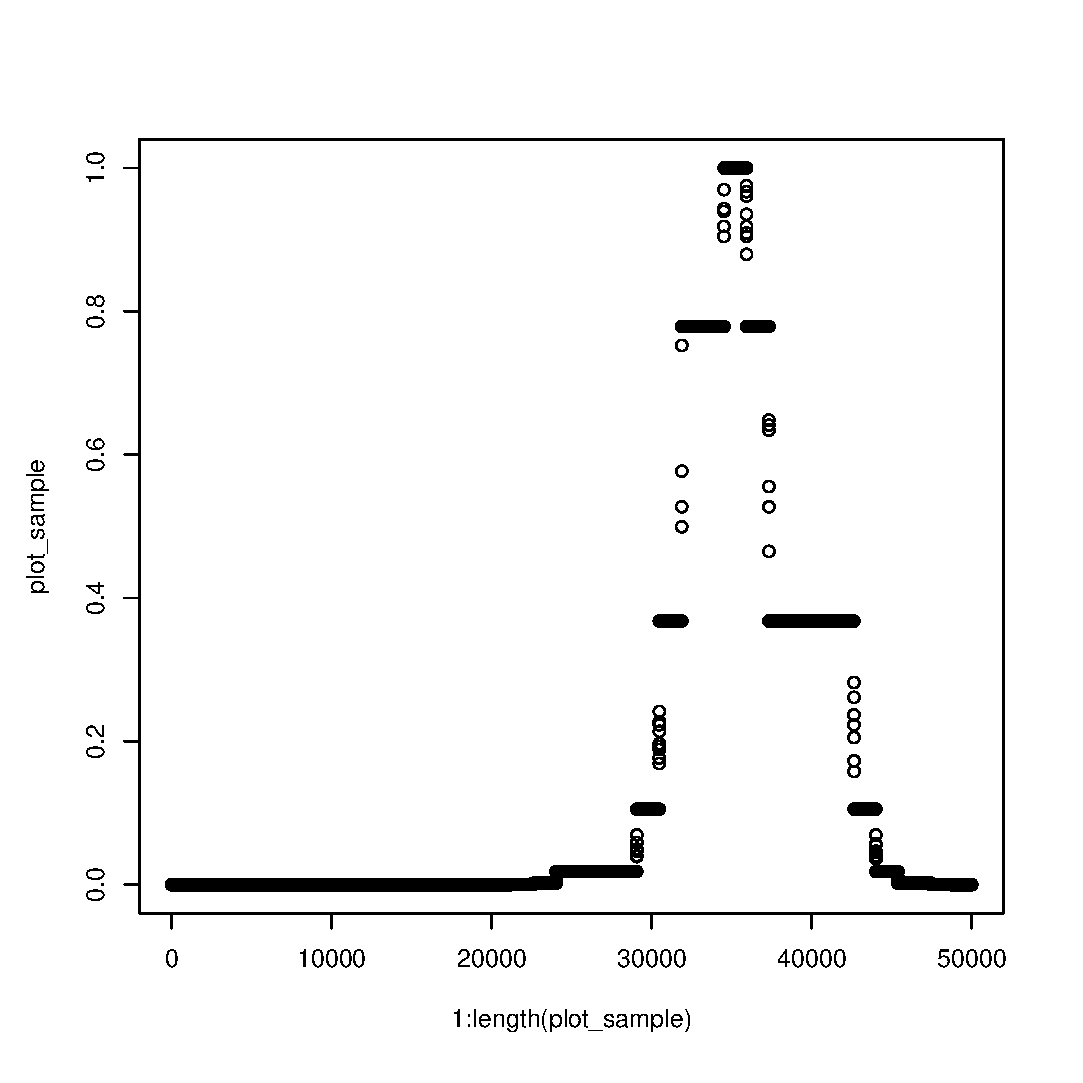
\includegraphics[width=\textwidth]{share/1_time.eps}
	    \end{minipage}
	    \begin{minipage}[]{0.2\textwidth}
	    	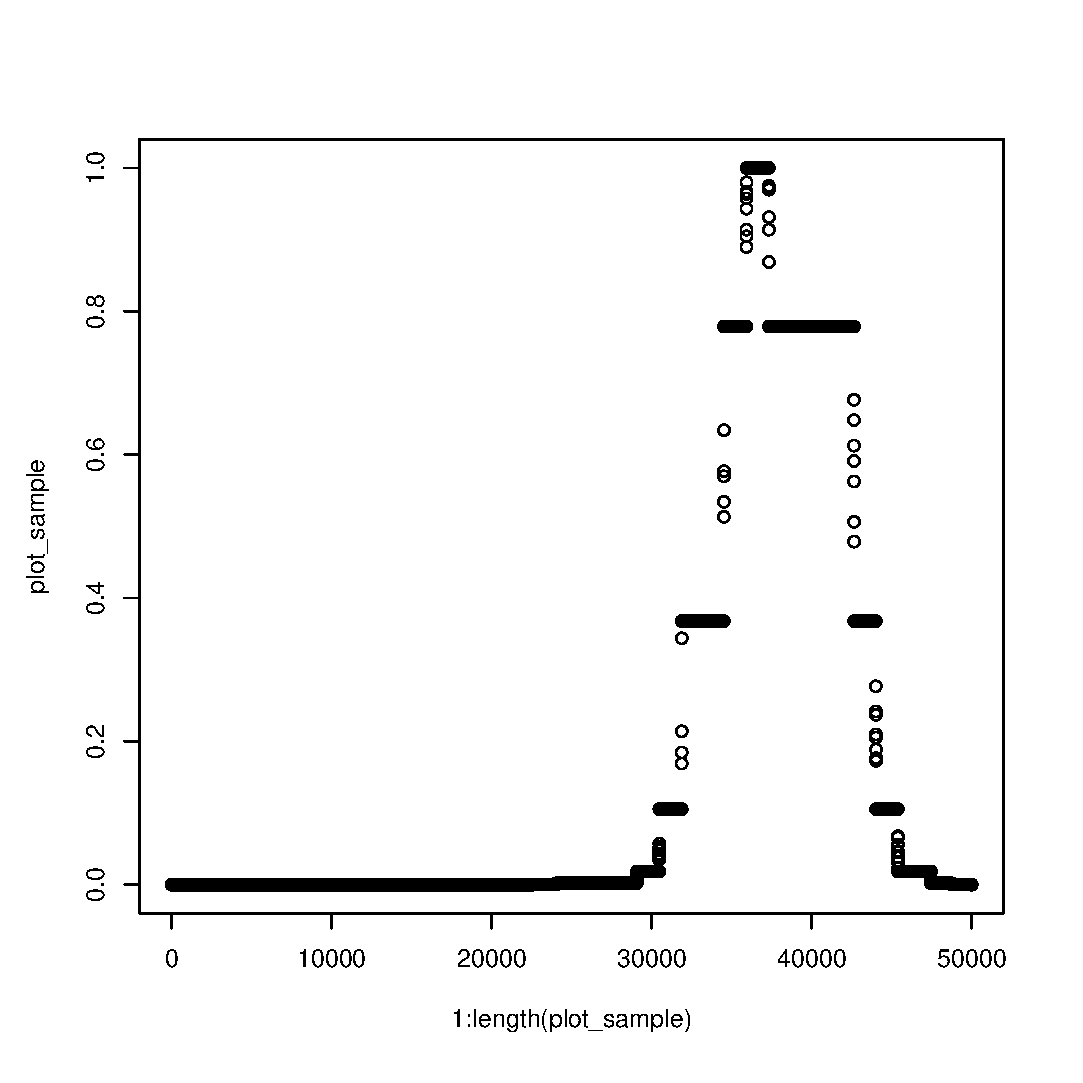
\includegraphics[width=\textwidth]{share/2_time.eps}
	    \end{minipage}
	    \begin{minipage}[]{0.2\textwidth}
	    	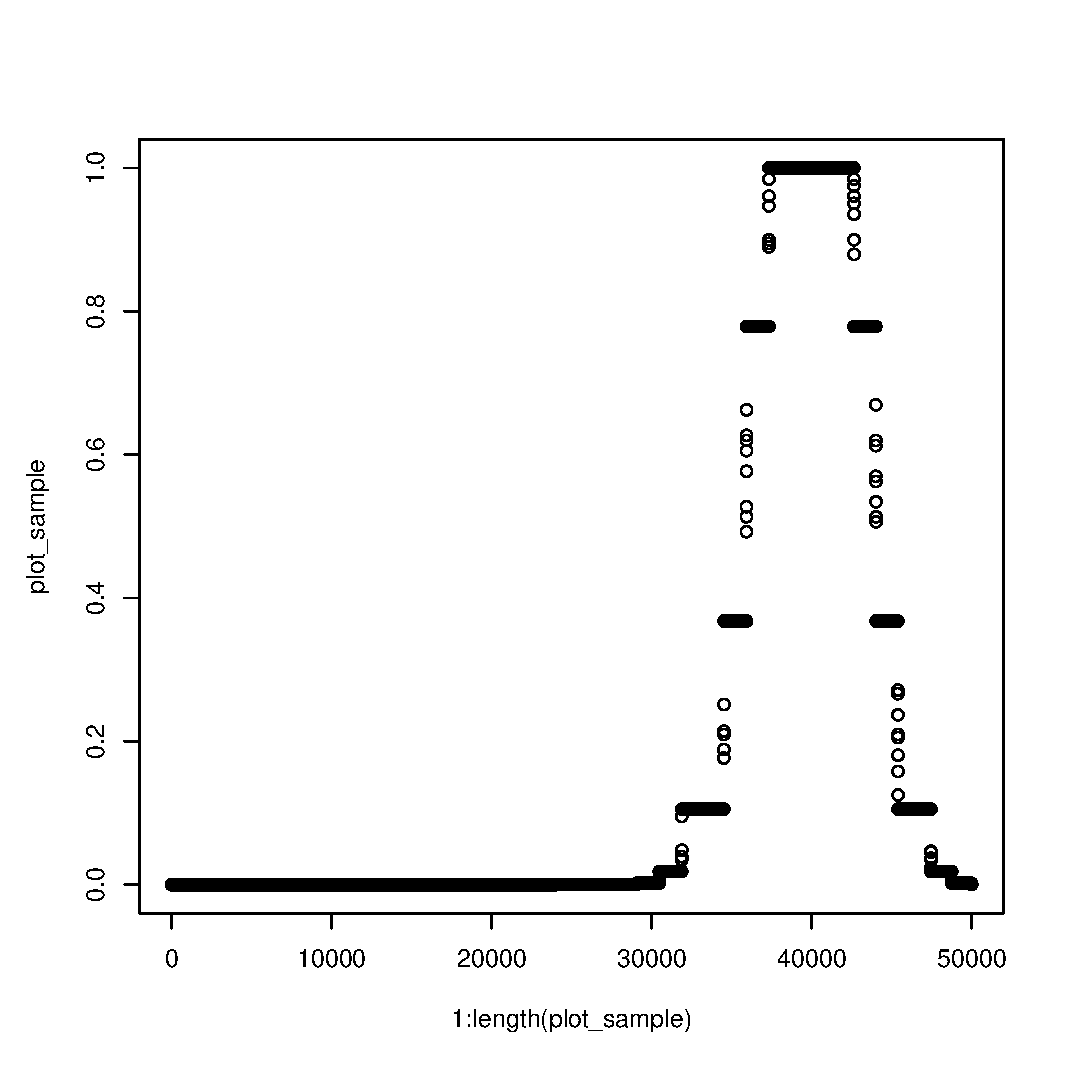
\includegraphics[width=\textwidth]{share/3_time.eps}
	    \end{minipage}
	    \begin{minipage}[]{0.2\textwidth}
	    	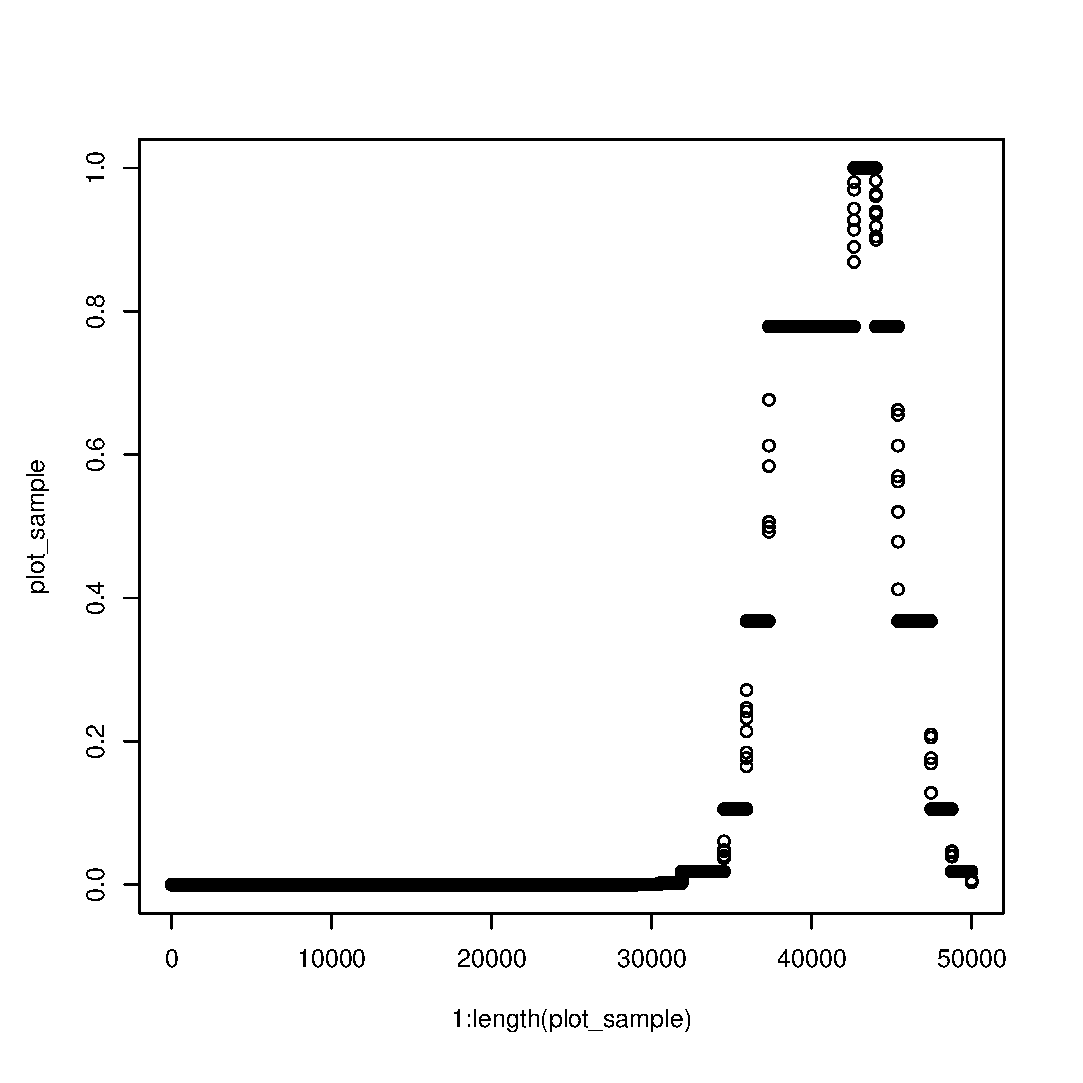
\includegraphics[width=\textwidth]{share/4_time.eps}
	    \end{minipage}
	    \begin{minipage}[]{0.2\textwidth}
	   		 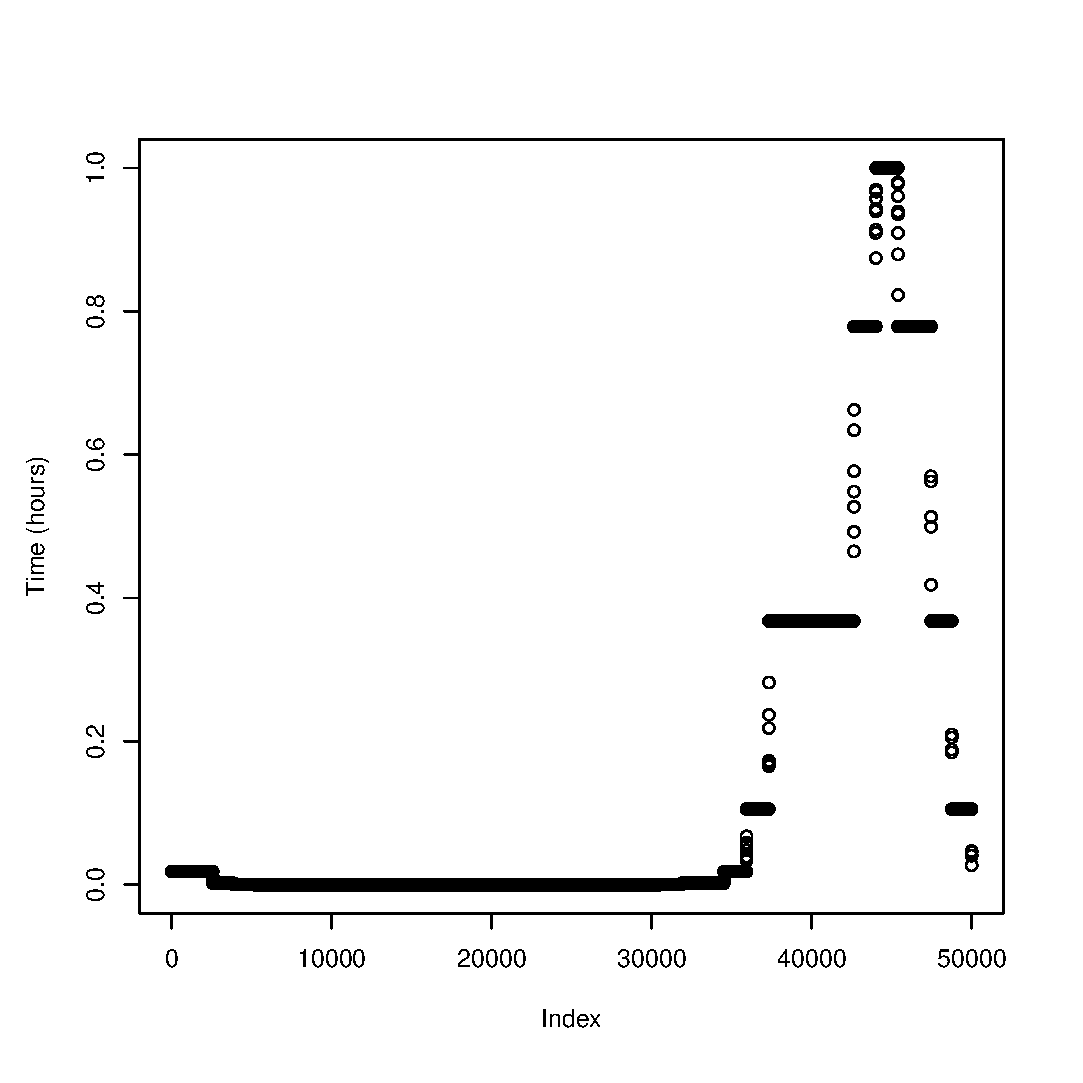
\includegraphics[width=\textwidth]{share/5_time.eps}
	    \end{minipage}
	    \begin{minipage}[]{0.2\textwidth}
	    	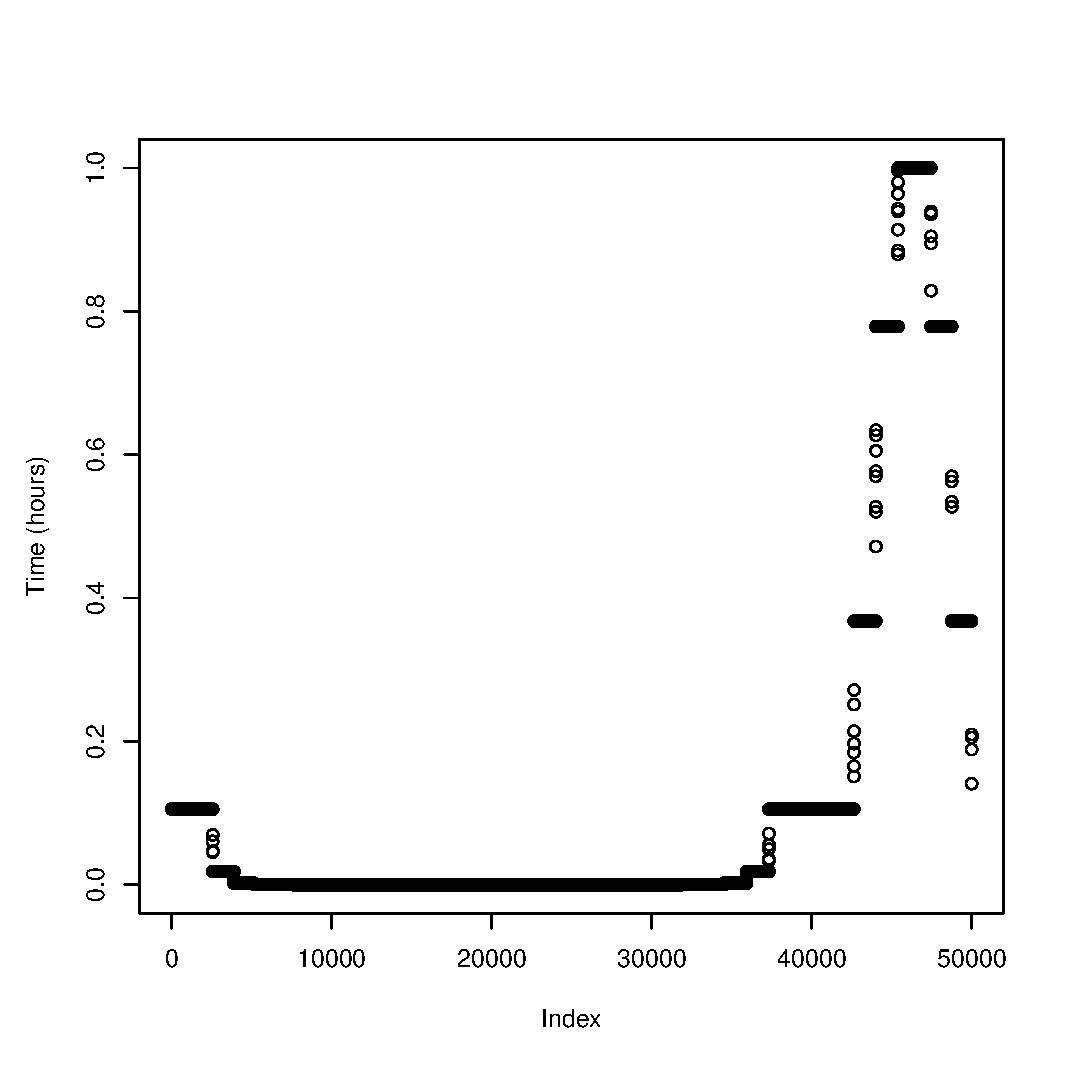
\includegraphics[width=\textwidth]{share/6_time.eps}
	    \end{minipage}
	    \begin{minipage}[]{0.2\textwidth}
	    	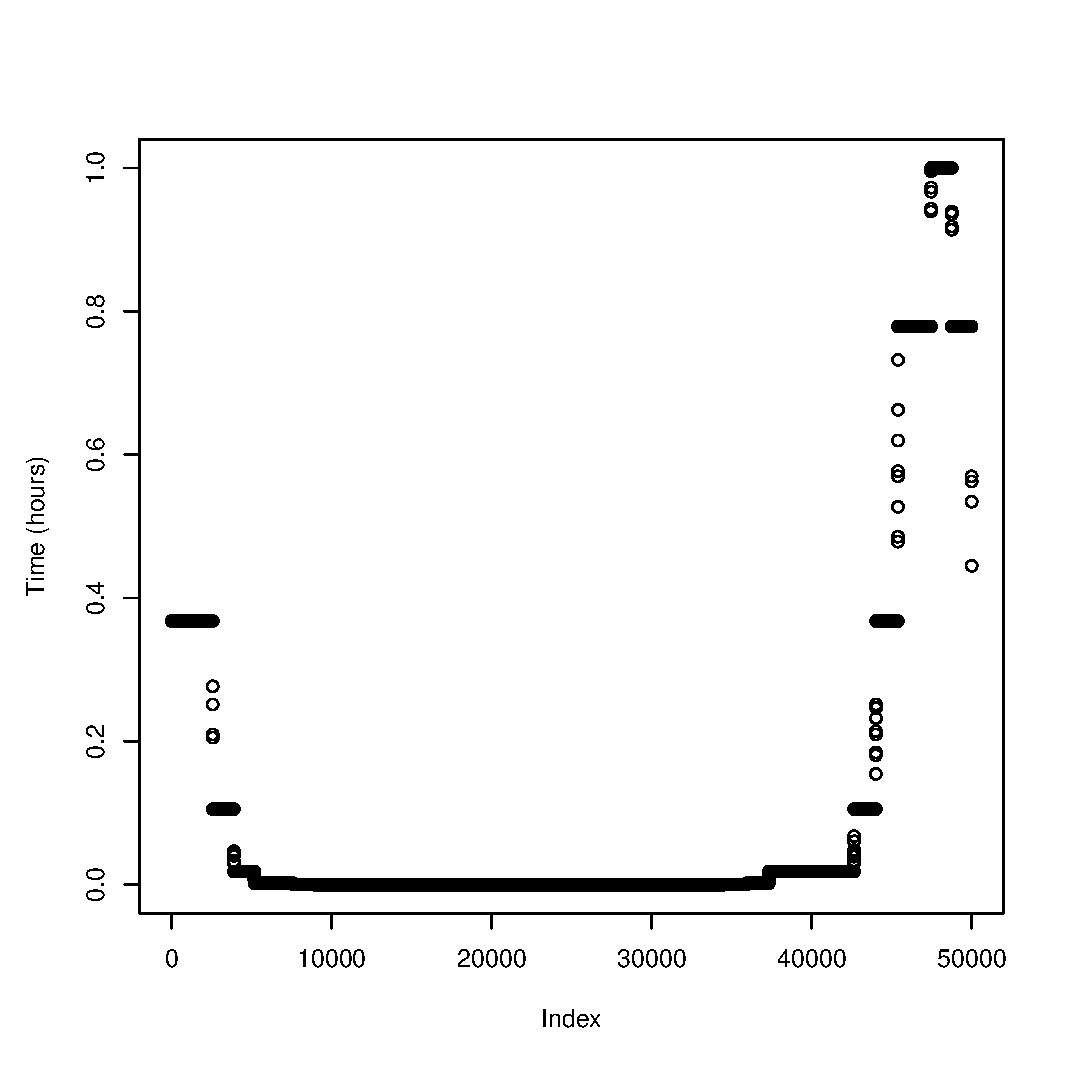
\includegraphics[width=\textwidth]{share/7_time.eps}
	    \end{minipage}
	    \begin{minipage}[]{0.2\textwidth}
	   		 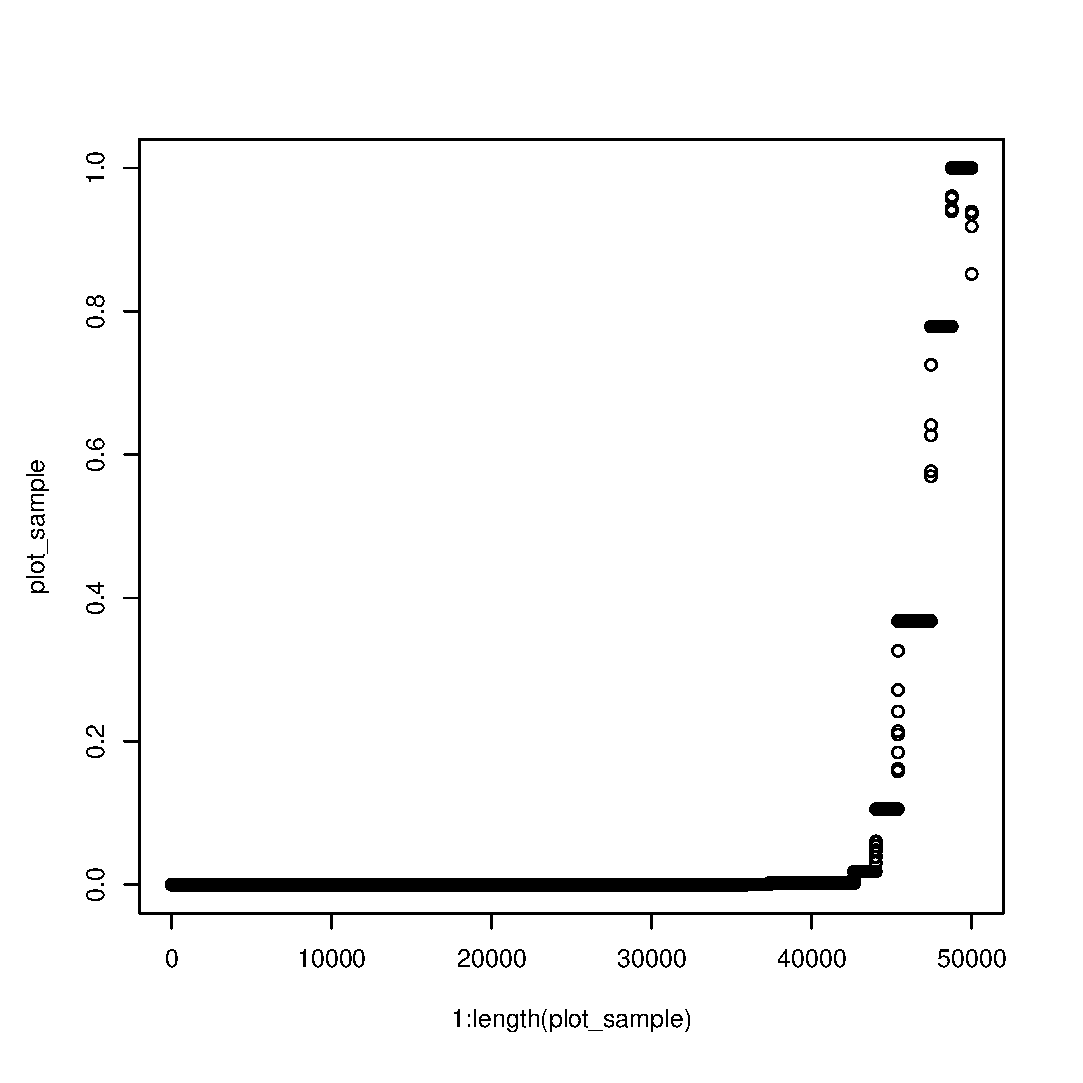
\includegraphics[width=\textwidth]{share/8_time.eps}
	    \end{minipage}
	    \begin{minipage}[]{0.2\textwidth}
	    	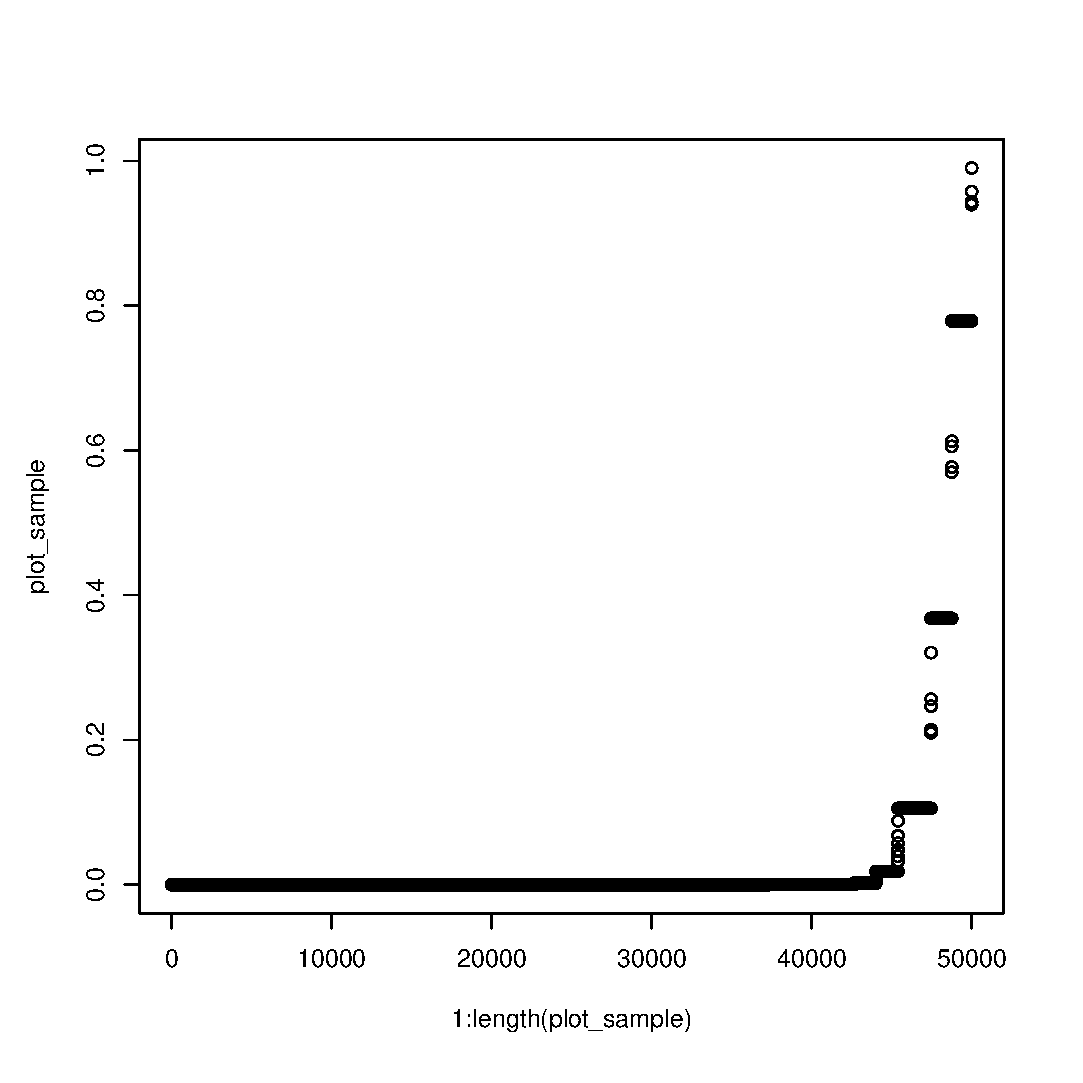
\includegraphics[width=\textwidth]{share/9_time.eps}
	    \end{minipage}
	    \begin{minipage}[]{0.2\textwidth}
	    	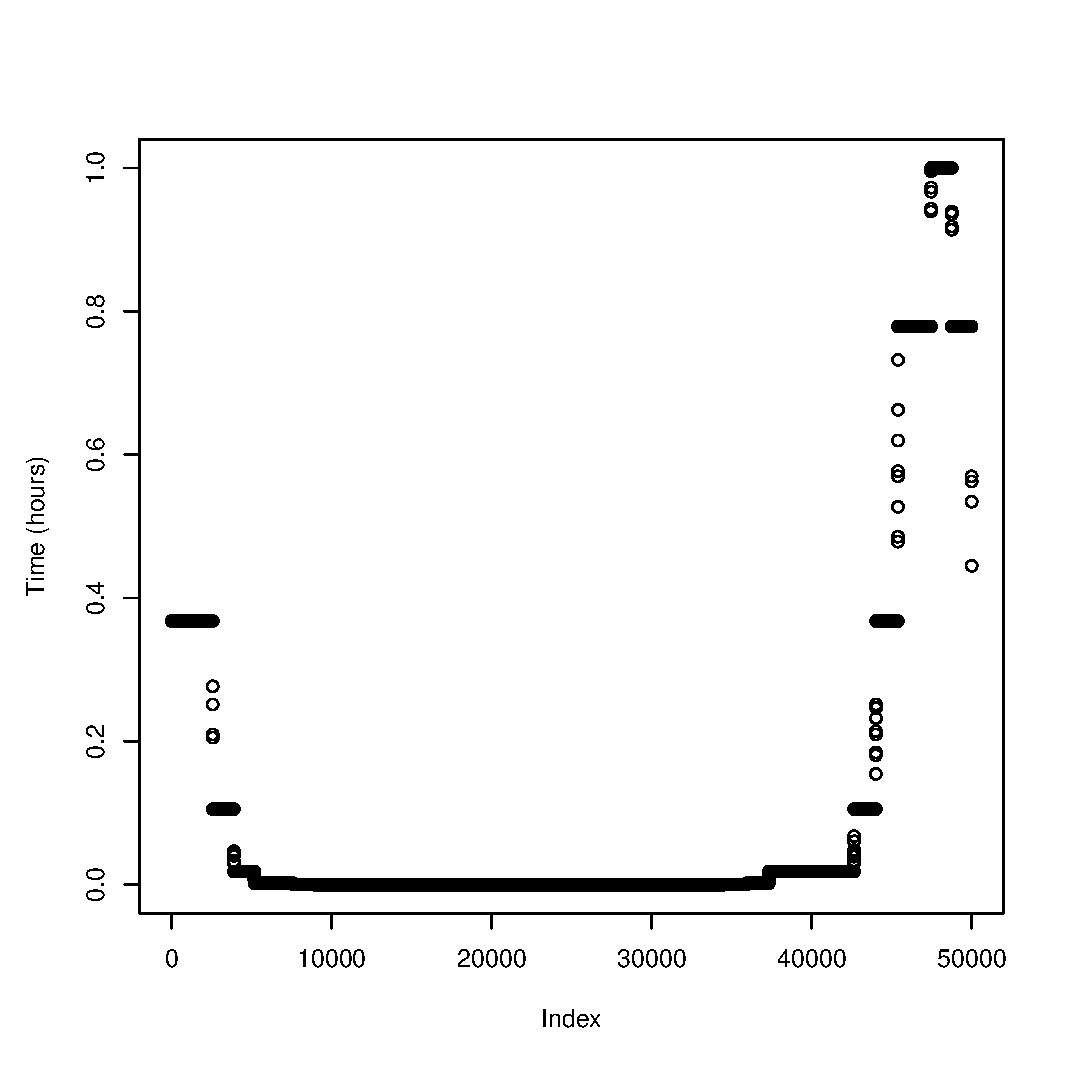
\includegraphics[width=\textwidth]{share/10_time.eps}
	    \end{minipage}
	    \begin{minipage}[]{0.4\textwidth}
	    	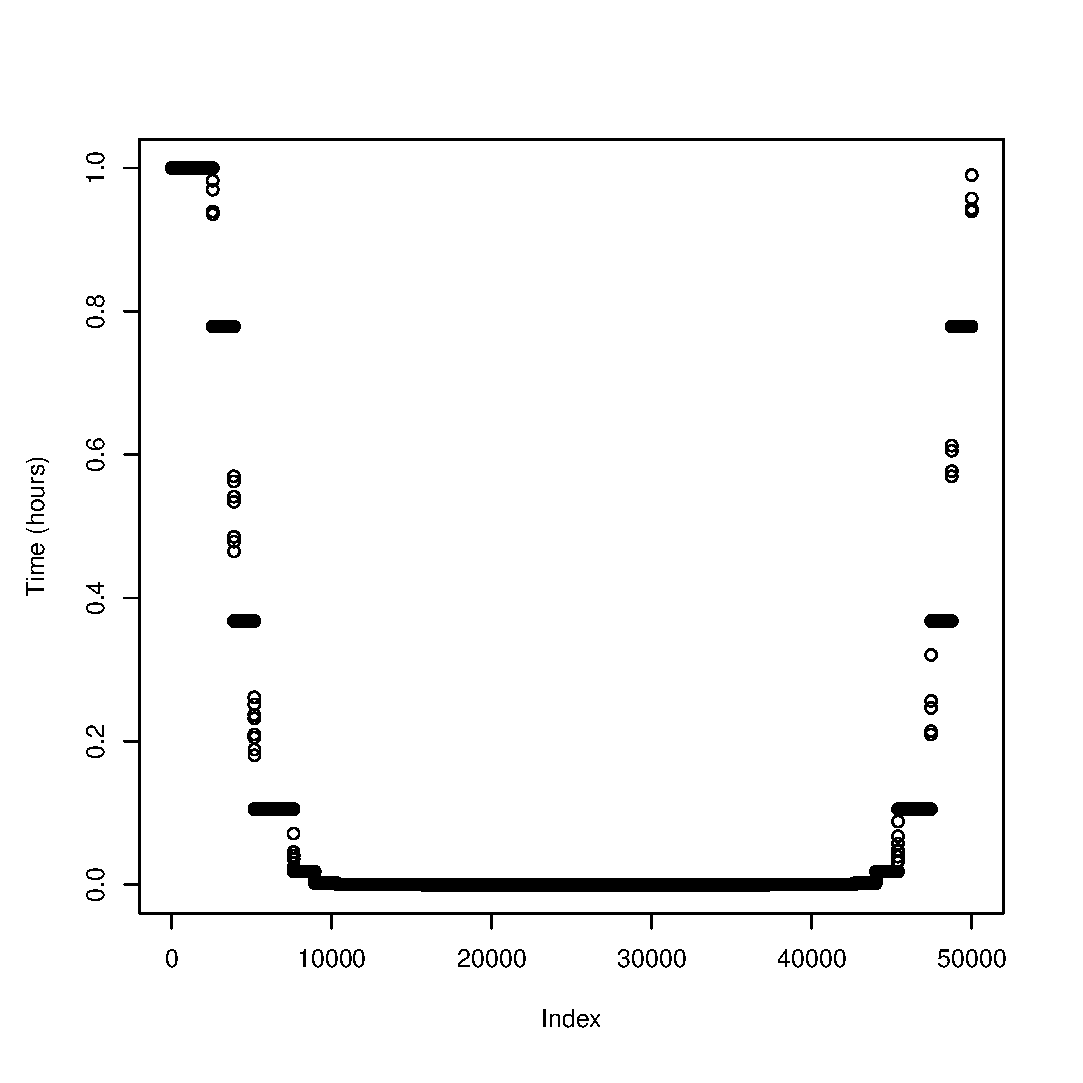
\includegraphics[width=\textwidth]{share/11_time.eps}
	    \end{minipage}
    \end{figure}

    \begin{figure}[H]
    \centering
    \caption{Distance plot (day of year) for the observations (Ordered by month/day)\label{fig:day}}
	    \begin{minipage}[]{0.4\textwidth}
	    	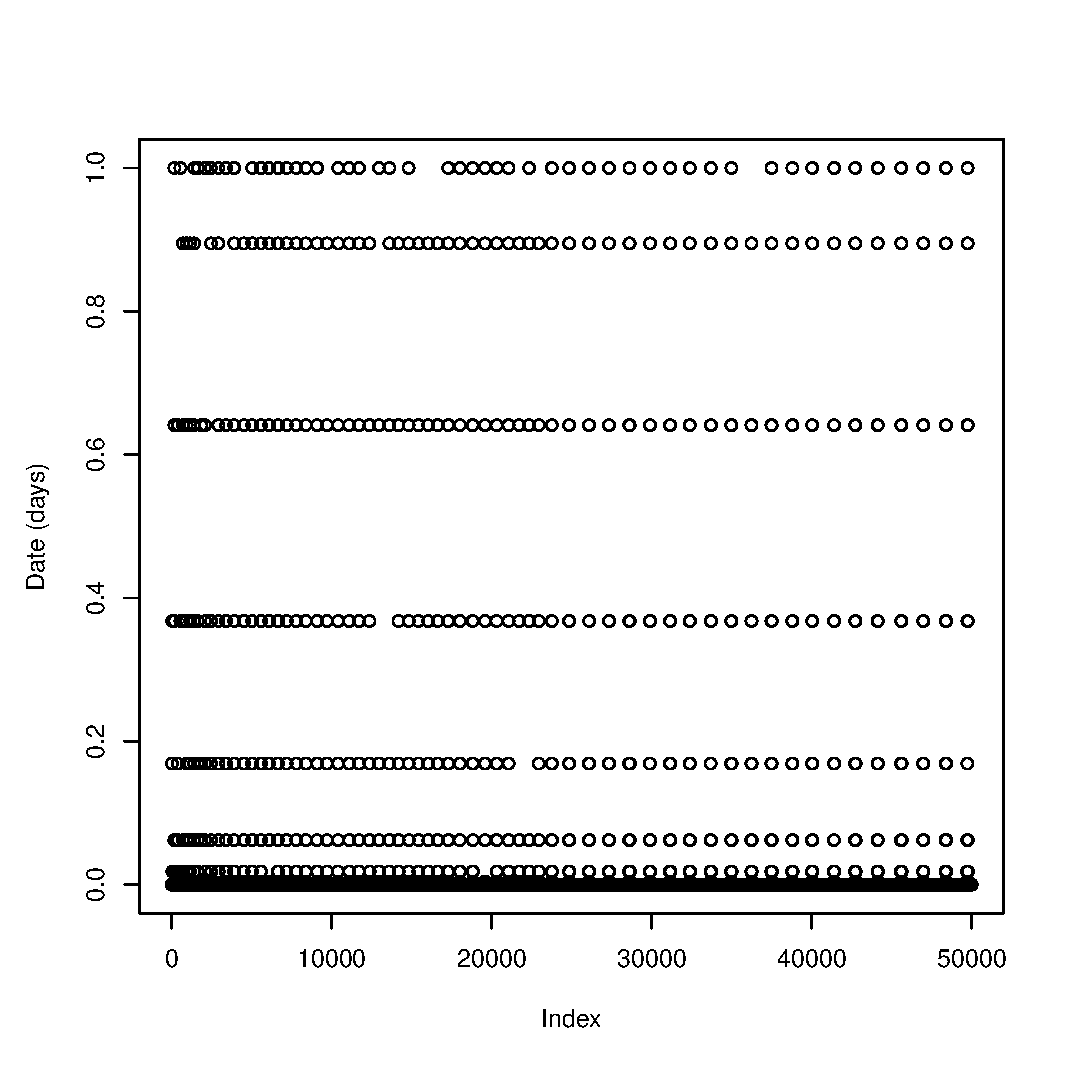
\includegraphics[width=\textwidth]{share/1_date.eps}
	    \end{minipage}
    \end{figure}

    \begin{figure}[H]
    \centering
    \caption{Distance plot (day of year) for the observations (ordered by station)\label{fig:dist}}
	    \begin{minipage}[]{0.4\textwidth}
	    	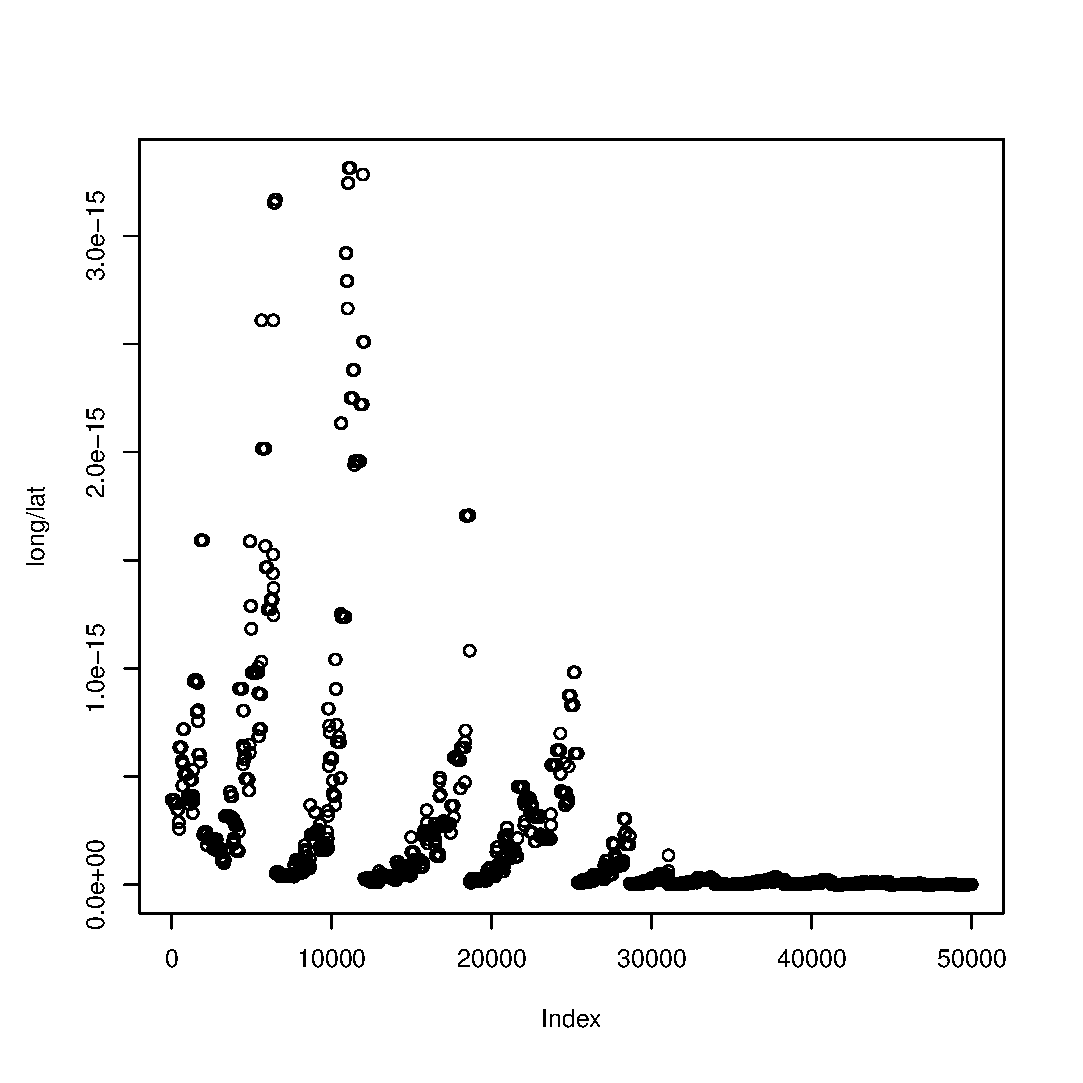
\includegraphics[width=\textwidth]{share/1_dist.eps}
	    \end{minipage}
    \end{figure}

    \begin{figure}[H]
    \centering
    \caption{Predicted temperature for the day 2013-04-12 in the interval 04:00-24:00 (ordered by hour)\label{fig:result}}
	    \begin{minipage}[]{0.4\textwidth}
	    	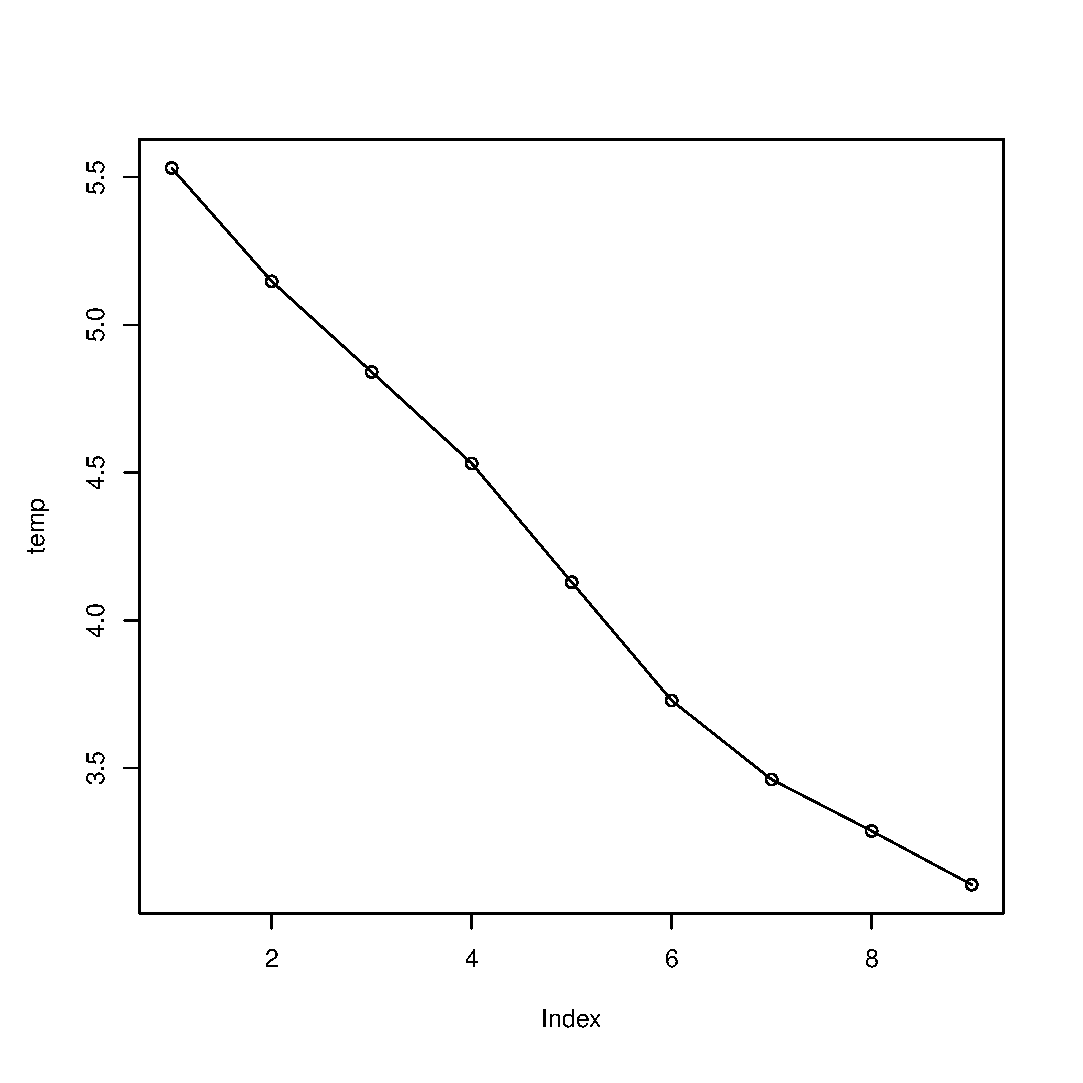
\includegraphics[width=\textwidth]{share/result.eps}
	    \end{minipage}
    \end{figure}


    \begin{figure}[H]
    \centering
    \caption{Predicted temperature for the day 2013-07-12 in the interval 04:00-24:00 (ordered by hour)\label{fig:bad_result}}
	    \begin{minipage}[]{0.4\textwidth}
	    	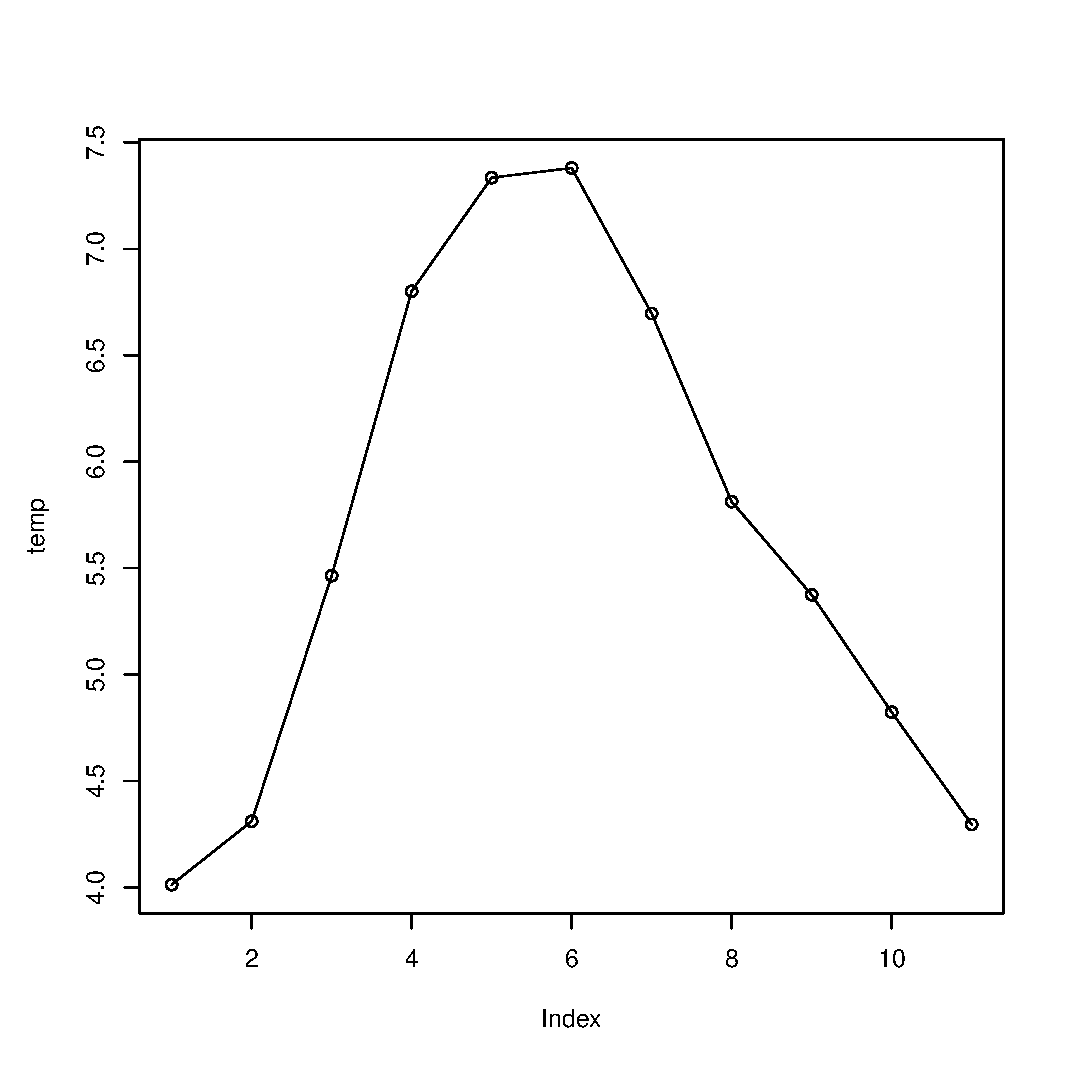
\includegraphics[width=\textwidth]{share/bad_result.eps}
	    \end{minipage}
    \end{figure}


    \nocite{*} % No warnings.
    \bibliographystyle{alpha}
    \bibliography{report}
    \onecolumn \appendix
    \section*{Appendix}
 	\lstinputlisting[caption={Script for Assignment},label={lst:script}]{../share/script.r}


    \end{document}
